\subsubsection*{Moments in time}
Moments in time \footnote{Moment,http://moments.csail.mit.edu/TPAMI.2019.2901464.pdf} คือชุดข้อมูลที่ใช้มนุษย์ในการ label ทั้งหมดให้กับวิดีโอสั้นถึง 1 ล้านวิดีโอ และมีจำนวน activity หรือกระทำต่างกัน 339 class โดยแต่ละวิดีโอจะมีความยาวอยู่ที่ 3 วินาที เนื่องจากเป็นเวลาเฉลี่ยที่มนุษย์ใช้ในการเข้าใจกับเหตุการณ์ที่เกิดขึ้น (human working memory) รูปแบบของชุดข้อมูลจะมีอยู่ทั้งหมดอยู่ 3 รูปแบบ ได้แก่ ภาพนิ่ง (spatial) เสียง (auditory) และการเคลื่อนไหว (temporal) นอกจากนี้ชุดข้อมูลนี้นั้นไม่รวบรวมเพียงแค่การกระทำของมนุษย์เท่านั้น ยังรวมไปถึง สัตว์ สิ่งของ และ ปรากฏการณ์ธรรมชาติ ทำให้ ชุดข้อมูลนี่เป็นการท้าทายรูปแบบใหม่เพราะด้วยข้อมูลที่มีความซับซ้อนมากขึ้น เช่น การสร้างโมเดลที่สามารถบอกถึงการกระทำ (action) ได้ถึงแม้ว่าสิ่งที่เราสนใจ (มนุษย์ สัตว์ สิ่งของ หรือปรากฏการณ์ธรรมชาติ) จะแตกต่างกัน เป็นต้น

\begin{figure}[!ht]
	\centering
	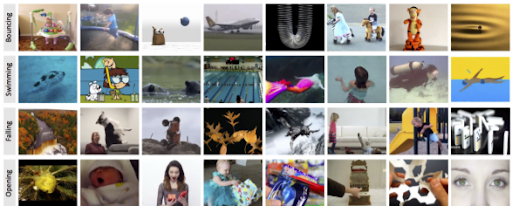
\includegraphics[width=1\textwidth]{chapter2/images/Example_of_class.png}
		\caption{ตัวอย่างของวิดีโอ class เดียวกันไม่จำเป็นต้องเป็น agents เดียวกัน}
    	\label{fig:moment_class}
\end{figure}

เป้าหมายของชุดข้อมูล Moments in time คือการออกแบบชุดข้อมูลให้มีความหลากหลาย ครอบคลุม ความสมดุล และจำนวนข้อมูลที่สูง โดยที่แต่ละ activity หรือการกระทำนั้นจะประกอบไปด้วยวิดีโอมากกว่า 1,000 วิดีโอ และมีการออกแบบมาเพื่อให้สามารถพัฒนาต่อได้ เช่น จำนวน class และข้อมูลภายใน class นั้น ๆ

\clearpage
\subsubsection*{1. วิธีการรวบรวมข้อมูล}
เริ่มจากการรวบรวมคำ (verb) ที่มีการใช้อยู่ทั่วไปในชีวิตประจำวันมา 4,500 คำจาก VerbNet จากนั้นนำมาแบ่งกลุ่มคำ(verb) ที่มีความหมายใกล้เคียงกันโดยใช้ features จาก Propbank และ FrameNet โดยเก็บข้อมูลเป็นแบบ binary feature vector ซึ่งถ้าคำ (verb) ไหนมีความเกี่ยวข้องกับ feature ก็จะให้ค่าเป็น 1 ถ้าไม่เกี่ยวข้องกันจะให้ค่าเป็น 0 จากนั้นจึงใช้วิธี k-means clustering ในการแบ่งกลุ่ม เมื่อแบ่งกลุ่มแล้วจากนั้นจะเลือกคำ (verb) จากในแต่ละกลุ่มนั้น โดยคำ (verb) ที่เลือกมานั้นจะเป็นที่ใช้บ่อยที่สุดในกลุ่มนั้น และลบคำ (verb) นั้นออกจากกลุ่มทั้งหมด (คำ ๆ หนึ่งสามารถอยู่ได้หลายกลุ่ม) จากนั้นจะทำกระบวนการนี่ไปเรื่อย ๆ แต่คำ (verb) ที่เลือกมาจะต้องไม่มีความหมายคลุมเครือ ไม่สามารถมองเห็นหรือได้ยินได้ และต้องไม่มีความหมายเหมือนกับคำ (verb) ที่เคยเลือกมาก่อน จนสุดท้ายแล้วได้ออกมาที่ 339 class
\par
ต่อมาทำการหาชุดข้อมูลวิดีโอโดยจะตัดออกมาเพียง 3 วินาทีที่เกี่ยวข้องกับคำ (verb) ใน 339 class ที่เลือกมา จากวิดีโอ แหล่งต่างกัน 10 แหล่ง การตัดวิดีโอนั้นจะไม่ใช้พวก Video2Gif (โมเดลที่ระบุตำแหน่งของสิ่งที่น่าสนใจในวิดีโอ) เพราะจะทำให้เกิด bias ขึ้นจะเกิดขึ้นตอนสร้างโมเดลจากนั้นจะทำการส่งข้อมูลของคำ (verb) และวิดีโอที่ตัดไปยัง Amazon Mechanical Turk (AMT หรือตลาดแรงงาน) เพื่อทำการ label โดยพนักงานแต่ละคนของ AMT จะได้ 64 วิดีโอซึ่งเกี่ยวข้องกับคำ (verb) หนึ่ง และอีก 10 วิดีโอที่มีการทำ label อยู่แล้ว โดยวิดีโอที่มีการทำ label ถ้ามีพนักงานของ AMT ตอบเหมือนกันกับที่ทำ label ไว้เกิน 90\% ถึงจะนำเข้าไปรวมกับชุดข้อมูลส่วนอีก 64 วิดีโอถ้าเป็นของ training set จะต้องผ่านพนักงานของ AMT อย่างน้อย 3 ครั้ง และต้อง label เหมือนกัน 75\% ขึ้นไปถึงจะถือว่าเป็น label ที่ถูกต้อง ถ้าเป็นของ validation และ test set จะต้องผ่านพนักงานของ AMT อย่างน้อย 4 ครั้ง และต้อง label เหมือนกัน 85\% ขึ้นไป ที่ไม่ตั่งเกณฑ์ไว้ที่ 100\% เพราะจะทำให้วิดีโอนั้นยากเกินไปที่จะทำให้สามารถจำการกระทำได้

\begin{figure}[!ht]
	\centering
	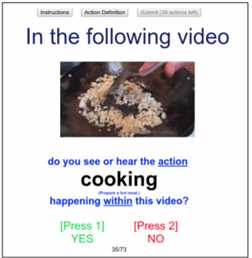
\includegraphics[width=0.5\textwidth]{chapter2/images/UI.png}
		\caption{User interface ของโปรแกรมทำ label}
    	\label{fig:User interface}
\end{figure}
\clearpage
\subsubsection*{2. ข้อมูลของ Moments in time}
มีวิดีโอมากกว่า 1 ล้านวิดีโอ และมี class ถึง 339 class ที่แตกต่างกัน มีค่าเฉลี่ยวิดีโอของแต่ละ class อยู่ที่ 1,757 และค่า median อยู่ที่ 2,775

\begin{figure}[!ht]
	\centering
	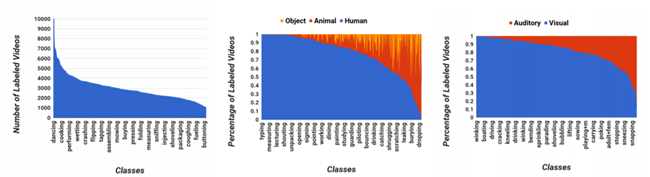
\includegraphics[width=1\textwidth]{chapter2/images/statistic_moment.png}
		\caption{สถิติของชุดข้อมูลของ Moments in timel}
    	\label{fig:statistic_moment}
\end{figure}
\subsubsection*{3. วิธีการทดสอบชุดข้อมูลและผลลัพธ์ที่ได้}
โดยการทดสอบแรกจะเป็นการทดสอบเทียบกับชุดข้อมูลอื่นดังภาพด้านล่าง

\begin{figure}[!ht]
	\centering
	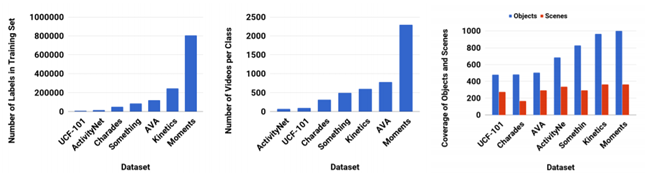
\includegraphics[width=1\textwidth]{chapter2/images/compare_dataset.png}
		\caption{เปรียบเทียบขอมูลระหว่างชุดข้อมูล}
    	\label{fig:compare_dataset}
\end{figure}

จากภาพจะเห็นได้ว่า Moments in time นั้นมีฉากหรือสถานที่ที่เหมือน Places = 100\% และมีวัตถุเหมือนกับ ImageNet ถึง 99.9 \%. ส่วนชุดข้อมูลที่มีความได้เคียงกับ Moments in time มากที่สุดคือชุดข้อมูล Kinetics ที่มีฉากหรือสถานที่ที่เหมือน Places = 99.5\% และมีวัตถุเหมือน ImageNet ถึง 96.6\%
\par
การทดสอบต่อมาจะเป็นการนำ Moments in time มาทดสอบสร้างโมเดลด้วยวิธีต่าง ๆ โดยจะเริ่มจากการเตรียมข้อมูลข้อมูลดังนี้
\begin{enumerate}
	\setlength\itemsep{-0.25em}
	\item training set จะมี 802,264 วิดีโอ และมีวิดีโอในแต่ละ class อยู่ที่ 500 ถึง 5,000 วิดีโอ
	\item validation set จะมี 33,900 วิดีโอ และมีวิดีโอในแต่ละ class อยู่ที่ 100 วิดีโอ
	\item เริ่มการ preprocess จากแยกภาพRGB ออกมาจากวิดีโอ และทำการเปลี่ยนขนาดของภาพให้เป็น 340x256  pixel
	\item ใช้ TVL1 optical flow algorithm จาก opencv เพื่อลดข้อมูลรบกวนที่จะเกิดขึ้น
	\item ทำการแปลงค่าที่อยู่ใน optical flow ให้เป็นเลขจำนวนเต็ม(integer) เพื่อทำให้การคำนวณนั้นเร็วยิ่งขึ้น
	\item ปรับค่า displacement ใน optical flow ให้ค่าสูงสุดเป็น 15 ต่ำสุดเป็น 0 และทำการปรับขนาดให้เป็นช่วง 0-255
	\item เก็บข้อมูลออกมาในรูปแบบของ grayscale image เพื่อลดพื้นที่ ๆ ใช้เก็บข้อมูล
	\item แก้ปัญหาเรื่องการเคลื่อนไหวของกล้อง(camera motion) โดยการนำค่าเฉลี่ยของ เวกเตอร์(vector) ไปลบกับ displacement
	\item สุดท้ายจะเป็นสุ่มตัดภาพออกมาเพื่อเพิ่มจำนวนข้อมูล
\end{enumerate}
หลังจากการเตรียมข้อมูลเรียบร้อยแล้วจะนำข้อมูลเหล่านั้นมาสร้างโมเดลด้วยวิธีการต่าง ๆ ดังตารางด้านล่าง

\begin{table}[!ht]
\centering
\begin{tabular}{|c|c|c|c|}
		\hline
		{Model}&{Modelity}&{Top-1(\%)}&{Top-5(\%)}\\
		\hline
		Chance			& -				& 0.29		& 1.47						\\
		\hline
		ResNet50-scratch	& Spatial			& 23.65		& 46.76						\\
		ResNet50-Places		& Spatial			& 26.44		& 50.56						\\	
		ResNet50-ImageNet	& Spatial			& 27.16		& 51.68						\\
		TSN-Spatial		& Spatial			& 24.11		& 49.10						\\
		\hline
		BNIncepion-Flow		& Temporal		& 11.60		& 27.40						\\
		TSN-Flow			& Temporal		& 15.71		& 34.65						\\
		\hline
		SoundNet			& Auditory			& 7.60		& 18.00						\\
		\hline
		TSN-2stream		& Spatial+Temporal	& 25.32		& 50.10						\\
		TRN-Multiscale		& Spatial+Temporal	& 28.27		& 53.87						\\
		I3D 				& Spatial+Temporal	& 29.51		& 56.06						\\
		\hline
		Ensemble(SVM)		& S+T+A 			& 31.16		& 57.67						\\
		\hline
	\end{tabular}
	\caption{Classification accuracy ของ TOP-1 และ TOP-5}
	\label{tab: Classification accuracy ของ TOP-1 และ TOP-5}
\end{table}

จากภาพจะเห็นได้ว่าผลลัพท์ที่ดีสุดคือการทำ ensemble(SVM) ซึ่งเป็นรวมของโมเดล ReNet50-ImageNet, I3D และ SoundNet จากผลลัพท์จะเห็นค่าที่ได้ออกมาจาก ensemble(SVM)  มีค่าใกล้เคียงกับรูปแบบ spatial เพราะประสิทธิของภาพเคลื่อนไหว(temporal) และ เสียง(auditory) นั้นมีประสิทธิภาพต่ำ ซึ่งจุดนี่จะทำให้เห็นว่าตัว Moments in time ยังทำให้สามารถพัฒนาต่อไปได้อีก
\par
ต่อมาจะทำทดสอบ cross dataset transfer โดยการนำโมเดล ResNet50 I3D pretrained ลงทั้งบน Kinetics และ Moments in time และนำมาเทียบกับชุดข้อมูลอื่น โดยชุดข้อมูลแต่ละชุดจะมีการปรับ frame rate ของวิดีโอให้เป็น 5 fps เหมือนกัน

\begin{table}[!ht]
	\centering
	\begin{tabular}{|c|c|c|c|}
		\hline
		{Pretrained}&\multicolumn{3}{c|}{Fine-Tuned}\\
		\cline{2-4}
		{}			& UCF		& HMDB		& Something			\\
		\hline
		\multirow{2}{*}{Kinetics}		& Top-1 : 92.6		& Top-1 : 62.0		& Top-1 : 48.6		\\
		{}						& Top-5 : 99.2		& Top-5 : 88.2		& Top-5 : 77.9		\\
		\hline
		\multirow{2}{*}{Moments}		& Top-1 : 91.9		& Top-1 : 65.9		& Top-1 : 50.0		\\
		{}						& Top-5 : 98.6		& Top-5 : 89.3		& Top-5 : 78.8		\\
		\hline
	\end{tabular}
	\caption{Data transfer performance ของโมเดล Resnet50 I3D}
	\label{tab: Data transfer performance ของโมเดล Resnet50 I3D}
\end{table}

จะเห็นได้ว่า Kinetics ให้ผลลัพท์ที่ดีกว่าใน UCF เพราะว่ามีการแชร์ class ด้วยกันอยู่หลายอย่าง ในขณะที่ HMDB นั้นมีการรวบรวม source จากหลายแหล่ง และมีจำนวน class ที่หลากหลายจึงทำให้มีความใกล้เคียงกับตัวข้อมูลของ Moments in time ดังนั้นจึงเทียบผลลัพท์จาก Something ซึ่งจะทำให้เห็นว่า Moments in time มีประสิทธิภาพที่ดีกว่าและวิดีโอที่มีความยาวมากกว่า 3 วินาทีจะไม่ส่งผลกระทบกับประสิทธิภาพของ Moments in time

\subsubsection*{4. ปัญหาที่พบ}
ผลลัพท์จากการทำนายด้วยโมเดลถ้าผ่านรูปภาพที่มีรายละเอียดเยอะจะทำให้การ ทำนายโอกาสผิดนั้นค่อนข้างสูง ซึ่งปัญหานี่สามารถทำให้เกิดน้อยลงด้วยการนำวิธี Class Activation Mapping(CAM) จะเป็นการเน้นรูปภาพในส่วนที่มีข้อมูลมากที่สุดและ ทำนายผลออกมา แต่ก็ยังมีจุดที่เป็นปัญหาอยู่ เช่น การกระที่เกิดขึ้นเร็วมาก (การลื่นล้ม) จะทำให้การทำนาย นั้นมีโอกาสผิดสูงขึ้น 

\begin{figure}[!ht]
	\centering
	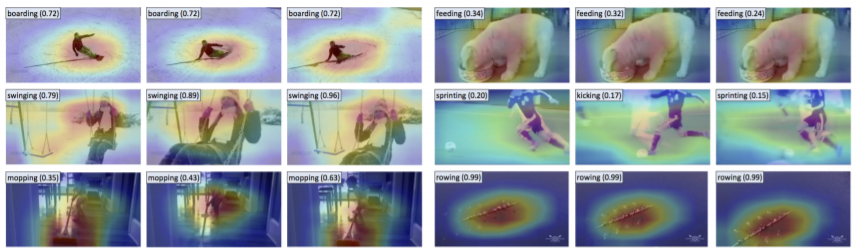
\includegraphics[width=1\textwidth]{chapter2/images/CAM.png}
		\caption{ภาพที่ได้จากการทำ CAM และผลลัพท์ที่ได้จากการทำนายด้วยโมเดล resnet50-ImageNet}
    	\label{fig:CAM}
\end{figure}


